\documentclass[10pt]{examdesign}
\usepackage{amsmath}
\usepackage{enumitem}
\usepackage{amsfonts}
\usepackage{pgfplots}
\usepackage{pifont}
\usepackage{graphicx}
\usepackage{fancyhdr}
\usepackage{cancel}
\usepackage{gensymb}
\usepackage[american]{circuitikz}

\SectionFont{\large\sffamily}
\Fullpages
\ContinuousNumbering
\usepackage{ulem}
\ProportionalBlanks{2}


\DefineAnswerWrapper{}{}
\NumberOfVersions{1}
%\IncludeFromFile{foobar.tex}
\examname{\Large{Impulse and Momentum}}
\class {\Large Physics}

\def \namedata {Name: \hrulefill\\ 
	Date: \hrulefill \\
	Period: \hrulefill \\
	Primary Peer Reviewer: \hrulefill 
	\\
			\begin{tabular}{| p{1cm} | p{1cm} | p{1 cm} | p{1cm} |}
	\hline
		+1 & 0 & -1 & $\Sigma$ 
		\\
		\hline
		& & & \vspace{.5cm}
		\\ \hline
	
	\end{tabular}
	\\
 \vspace{-.6in}
	
}




\begin{document}




\begin{multiplechoice} [title={Multiple Choice},
	rearrange=no]

\textit{For Each question, choose the best answer.}

	Some Formulas: 
	\begin{center}
	$\vec{J} = \vec{F} t $ \hspace {1in} $	\vec{p} = m \vec{v} $ \hspace{1in} 	$\vec{p_i} + \vec{J} = \vec{p_f}$
	\vspace{0.1in}
\end{center}	
	


\begin{question}
Which of the following statements is true concerning the relationship between kinetic energy and momentum?
\choice{If an object has non-zero kinetic energy, it has non-zero momentum.}
\choice{An object could have zero kinetic energy, but still have momentum.}
\choice{An object could have zero momentum, but still have non-zero kinetic energy.}
\choice{There is no relationship between kinetic energy and momentum.}
\end{question}

\begin{question}
Which of the following has the largest momentum relative to Earth?
\choice{a tightrope walker crossing Niagara Falls}
\choice{a pickup truck speeding along a highway}
\choice{an 18-wheeler parked in a lot}
\choice{a dog running down the street}
\end{question}

\begin{question}
	A clay ball and a rubber ball of the same mass are moving toward a glider that is at rest on a frictionless air track. The balls have the same speed, with the rubber ball moving toward the right and the clay ball moving toward the left, as shown above. The balls strike the glider at the same time. The clay ball sticks to the glider, and the rubber ball bounces off it. Which of the following indicates the direction of motion of the glider after the collisions and explains why it moves in that direction?
	
	\begin{center}
		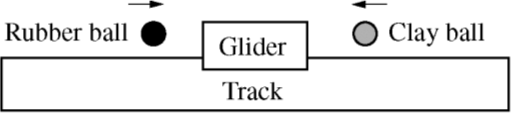
\includegraphics[height=0.4in]{glider.png}
	\end{center}

	
	\choice{The glider moves to the right because the magnitude of the change in momentum of the rubber ball is greater than the magnitude of the change in momentum of the clay ball.}
	\choice{The glider moves to the right because the collision with the rubber ball is elastic and conserves energy.}
	\choice{The glider moves to the left because the clay ball has more inertia when it sticks to the glider than the rubber ball does when it bounces off.} 
	\choice{The glider moves to the left because the clay ball exerts a force on the glider for a longer time than the rubber ball does.}



\end{question}



\begin{question}
A 2 kg object traveling at 5 m/s on a frictionless horizontal surface collides head-on with and sticks to a 3 kg object initially at rest. Which of the following correctly identifies the change in total kinetic energy and the resulting speed of the objects after the collision?

\choice{Kinetic Energy: Increases \hspace {1in} Speed: 2 m/s}
\choice{Kinetic Energy: Increases    \hspace {1in}       Speed: 3.2 m/s}
\choice{Kinetic Energy: Decreases    \hspace {.97in}       Speed: 2 m/s}
\choice{Kinetic Energy: Decreases     \hspace {.97in}      Speed: 3.2 m/s}
\choice{Kinetic Energy: Stays the Same \hspace {.6in}    Speed: 2 m/s}
	
\end{question}


\end{multiplechoice} 

\begin{multiplechoice} [title={Multiple Correct Multiple Choice},
	rearrange=no] \textit{For Each of the following question, choose TWO answers.  No credit will be given for incorrect or partially correct answers.}
	
	\begin{question}
		A ball is rolling in the +x direction.  You kick the ball, which results in the ball rolling perfectly in the -y direction.  Which of the following statements about the impulse delivered to the ball are true? (CHOOSE TWO)
		\choice{The impulse in the X direction was positive.}
		\choice{The impulse in the X direction was negative.}
		\choice{The impulse in the X direction was zero.}
		\choice{The impulse in the Y direction was positive.}
		\choice{The impulse in the Y direction was negative.}
		\choice{The impulse in the Y direction was zero.}
		\end{question}
	
	\end{multiplechoice}


\begin{shortanswer}[title={Free Response}, rearrange=no]
	\begin{question} 
A train of mass $1.8\times10^7$kg is traveling at 10 m/s when it strikes a car stuck on the tracks of mass 1300kg. The car becomes stuck to the train.  Determine the final velocity of the train-car system. 
\vspace{1.5 in}
	\end{question}



\begin{question}
A 750 kg car is traveling south on Lee-Trevino at 12 m/s when it is hit by a 3000 kg bus traveling West on Montwood as 5 m/s.  If the bus comes to a complete stop during the collision,
\begin{enumerate}
	\item What is the final velocity of the car?
	\vspace{1in}
	\item At what angle (measured from south) does the car travel?  
\end{enumerate}


\end{question}

	
\end{shortanswer}





\end{document}


